% This file is part of the BallPeenHammer project.
% Copyright 2013, 2014 the authors.

\documentclass[12pt,letterpaper,preprint]{aastex}

\newcommand{\instrument}[1]{\textsl{#1}}
\newcommand{\rf}[1]{\textbf{RF: #1}}
\newcommand{\vect}[1]{\mathbf{#1}}
\newcommand{\HST}{\instrument{HST}}
\newcommand{\WFC}{\instrument{WFC3}}
\newcommand{\FLT}{\texttt{FLT}}
\newcommand{\data}{\vect{D}}
\newcommand{\model}{\vect{M}}
\newcommand{\bkg}{\vect{B}}
\newcommand{\psf}{\vect{\psi}}
\newcommand{\pixelpsf}{\vect{\Psi}}
\newcommand{\var}{\vect{\sigma}^2}
\newcommand{\gradients}{\vect{g}}

\begin{document}

\title{The \HST\ \WFC\ IR-channel point-spread function}
\author{Ross Fadely \& David W. Hogg}

\begin{abstract}
Accurate point-source photometry and astrometry depends on an accurate model of the point-spread function (PSF).
The publicly available models for the PSF in the \HST\ \WFC\ IR-channel instrument are not accurate.
Here we construct an empirical model of this PSF,
  using archival observations of compact sources taken with the instrument.
Our model is of the \emph{pixel-convolved} PSF;
  it is a model for the PSF as it appears in the pixel read-outs of the instrument
  as a function of the sub-pixel position of the source.
We build our model for the XXX, YYY, and ZZZ bandpasses;
  the PSF in other bandpasses can be interpolated from these.
The variation of the PSF with position in the focal plane
  is apparent in the model.
We don't explicitly model the dependence of the PSF on source color,
  but we show that there are effects evident in the data.
All the code is released under an open-source license
  and all the results are presented in machine-readable form.
\end{abstract}

\keywords{
  method:~statistical
}

\section{Introduction}

The imaging devices on the \instrument{Hubble Space Telescope} (\HST) are generally not well sampled,
  meaning that they do not have multiple pixels spanning the full-width half-maximum (FWHM)
  of the point-spread function (PSF).
In a space-based mission,
  good sampling is traded off against detector size, field-of-view, and telemetry bandwidth.
Sampling is often made lower in priority,
  especially since well-sampled images can be made by taking multiple
  ill-sampled images at partial-pixel dithers.
Poor sampling renders some image operations,
  like pixel interpolation, point-source astrometry, and identification of cosmic rays,
  substantially more difficult than they are in well-sampled images.

However, even if sampling is poor,
  the response of the device to a point source is nonetheless continuous in source position.
That is, it is possible, even for poorly sampled images,
  to make a prediction or model of the pixel brightnesses generated by
  a star of any brightness at any (precise, sub-pixel) position in the focal plane.
This prediction gets smoother as the sampling is improved,
  and the model gets less complex (less featured),
  but it can be made at any sampling, even very bad samplings.
There is nothing difficult in principle about making this prediction or model,
  nor in training it with real imaging of real stars taken with the device.
What's astonishing is that,
  for the incredibly productive and important \HST\ imaging instruments,
  this model has never (to our knowledge) been made (soften this?).
Here we address this by building, testing, and releasing such a model.

There are models of the \emph{optical PSF} of the \HST\ (cite TinyTim, anderson06);
  these are models of the light field falling on the detector pixels. \rf{there are WFC3 IR psfs build by Anderson and Dolphin}
The optical PSF is not directly observed in an image;
  what is observed is the pixel-convolved PSF---%
  the optical PSF integrated over a pixel---%
  which, when the imaging is poorly sampled,
  depends strongly on both the optical PSF
  and the detailed shape and sensitivity of the pixels.
What a data analyst wants is a model of the pixel-convolved PSF,
  which can be used directly to perform astrometric and photometric measurements on images,
  without additional assumptions about the pixels.
In addition to this ``unobservability'' of the optical PSF,
  there is the additional problem that the aforementioned optical PSF models
  are built not from the (abundant) data expensively telemetered down from the Satellite,
  but rather from theoretical models of the complicated optics.
We find that these optical PSF models are not only \emph{not} what we need in our data analyses,
  they are also inaccurate, probably because they haven't been forced to agree with the data.

In what follows we build an empirical or data-driven model
  of the pixel-convolved PSF for the \HST\ \WFC\ IR-channel imaging device.
Our model is novel in several respects:
It is based entirely on data;
  it is a flexible model of real data.
It is built using essentially all the available data from the instrument.
It accounts for dependences of the PSF on bandpass and focal-plane position.
It is a pixel-convolved PSF,
  so it predicts the pixel read-outs very directly and without convolution by any pixel model.
It extremely accurately predicts the pixel contents of real images.
It is built with open-source code,
  all of which is available for repurposing to other imagers on \HST\ or other space-based facilities.

\section{Data}

For this initial project, we focus on the F160W filter for the WFC3 IR channel.  Our goal is to build 
an accurate PSF model that is sufficiently complex to deliver precise photometry across the 
detector.  In order to facilitate this, we have acquired as much F160W images from the MAST 
archive that meet our criteria for use.  Our criteria for an image to be downloaded is simple: the 
images must be publicly available and have apertures that cover the full detector, namely they 
have apertures \texttt{IR}, \texttt{IR-FIX}, \texttt{IR-UVIS-CENTER}, or \texttt{IR-UVIS-FIX}.

Similar to \citet{anderson06}, we only use \FLT\ images for our analysis.  \FLT\ images are calibrated 
using the most recent models for the bias, flat field, CTE, etc, and for this work we assume there are 
no errors in these calibrations that will effect our PSF estimation.  We choose to work with \FLT\
images for many reasons.  Primarily, we choose not to work with Drizzled or combined images
because they introduce distortions to the underlying PSF that is not consistent across images, and 
they introduce strongly correlated noise.  Additional benefits of the \FLT\ data are that they are 
more numerous by a factor of a few, sources lie different positions on the detector due to dithering, 
and they are well calibrated.  

For each \FLT\ image, we extract high signal-to-noise objects which we believe to be stars.  There 
are many approaches to find such sources, for simplicity we choose the following horrifying hack 
procedure.  We run \texttt{SExtractor} \citep{bertin96} and extract the `stellarity' index and blending/error 
flags.  We call an object a `star' if it has stellarity greater than 0.8, has a peak pixel value greater than 25
times the median of the counts ($e^- / \rm{s}$) in the image, and has no SExtractor blending or 
error flags.  More sensible approaches to source finding exist, but visual inspection of the images 
show that these criteria generally point to high signal to noise starlike objects with little contamination.
When modeling these sources, we require that any pixel used in the model have no data quality 
flags other than zero (meaning no issues), as defined by the \texttt{DQ} extension in the \FLT\ file.  
The data we extract for each source is a 25 pixels by 25 pixels patch where the central pixel is defined
to be the brightest pixel in the data.  Figure \ref{fig:data-examples} shows 9 example patches from the 
extraction.

The properties of the \WFC\ IR detector, is such that electrons from previous and current exposures 
will `persist' in pixels, resulting in electron counts higher than provided by the source in question.  
The issue of persistences is mainly only troublesome for bright sources, where counts may be 
enhanced by \rf{a few} percent of the counts provided the illuminating source.  This is generally 
not an issue for the sources we consider here.  Nevertheless, we use the HST persistence 
model\footnote{http://archive.stsci.edu/prepds/persist/search.php} to subtract off any possible 
persistence in the observation.  For simplicity we assume that this model is error free.

In total, we extract sources from \rf{XXXX} images, which were download from a list constructed on 
\rf{DDMMYYYY.}  In total, we have $\sim1.8$ million sources which we deem to be starlike, distributed 
in a fashion close to Poisson across the detector.  Our Github repository contains a JSON list of the
observations downloaded.

\begin{figure}
\centering
 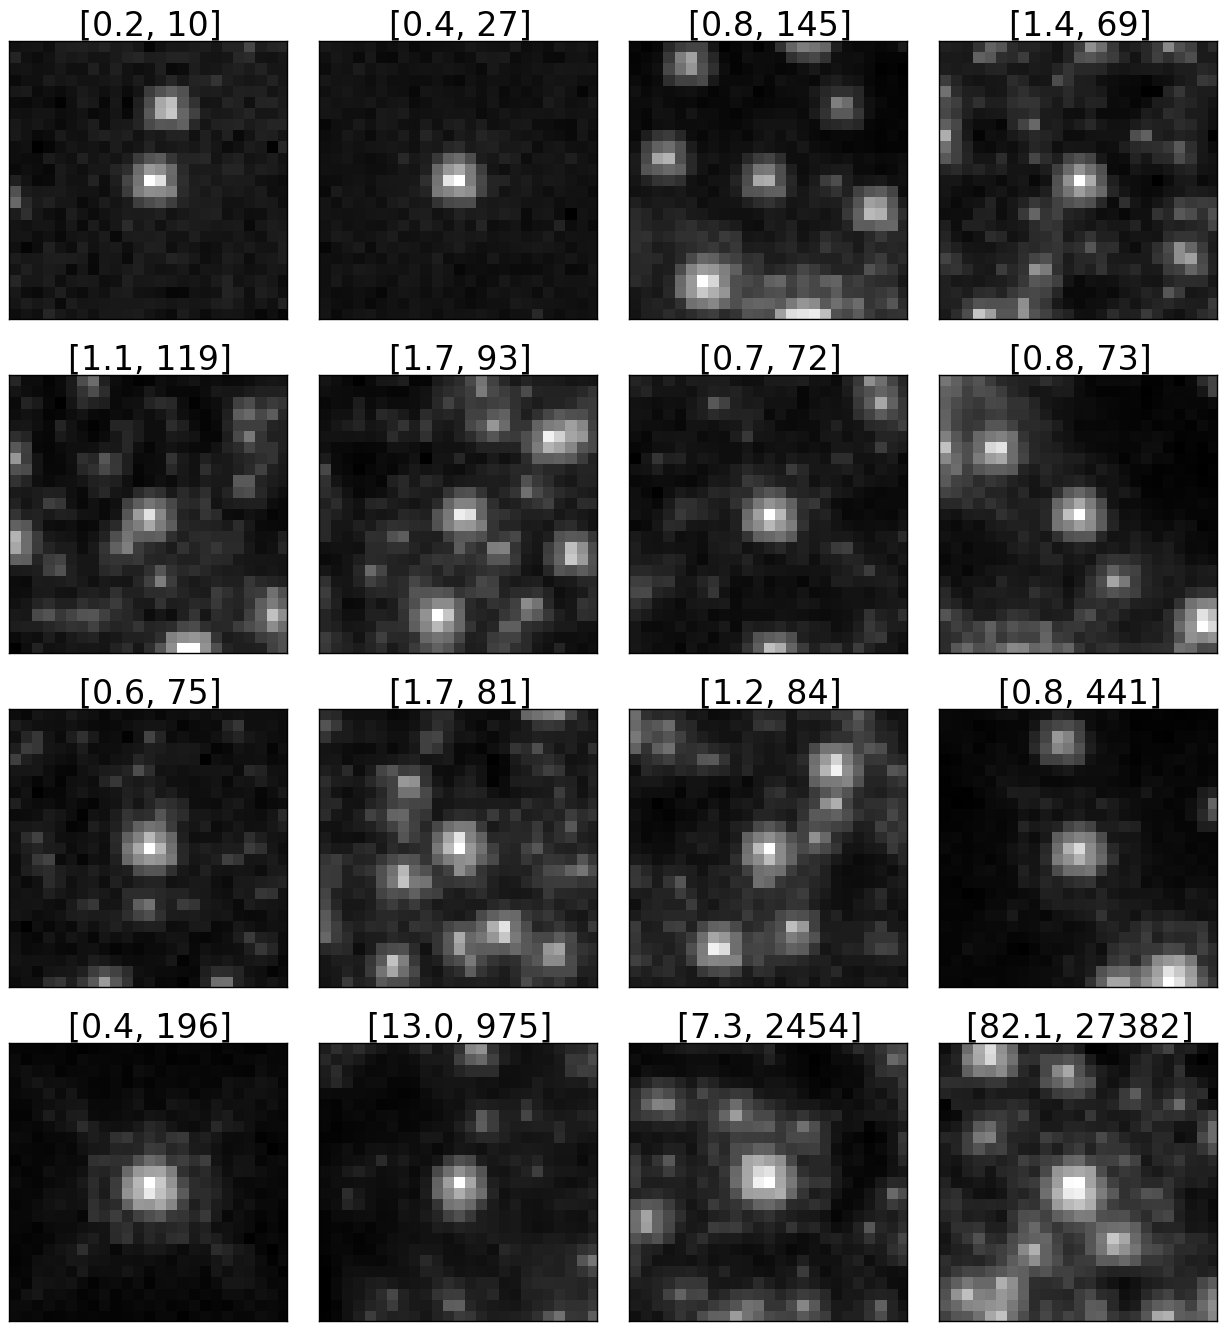
\includegraphics[clip=true, trim=0cm 0cm 0.0cm 0.cm,width=12cm]{../../plots/paper/fig1.png}
\caption{Example patches of size 25$\times$25 pixels from F160W \FLT\, images, displayed log-scaled.
Shown at the top left (bottom right) is the patch with smallest (largest) peak flux whose center falls within
100 from the center of the detector.  Other patches shown are randomly selected from the same sample.
Above each patch is the minimum and maximum pixel value contained in the patch.
It is clear that the majority of our patches come from observations of dense stellar fields, yet significant 
fractions of patches with isolated or fairly isolated stars are prevalent.}
\label{fig:data-examples}
\end{figure}



\section{Methodology}

\subsection{Source Model}
\label{ssec:model}

We model the intensity of the pixels in each data patch $\data_i$ as a single scaled PSF plus a constant value 
background flux.  That is we model the data as 

\begin{eqnarray}
\model_i =  A_i \psf_i + \bkg_i
\quad , 
\label{eqn:model-patch}
\end{eqnarray}

\noindent where $A_i$ is an amplitude that scales the normalized pdf model $\psf_i$ and $\bkg_i$ is 
the (constant) background for the patch.  

Do in part to the fact that the WFC3 PSF is undersampled,  it 
is important that the PSF for any patch be a function of the sub-pixel centroid of the star ($x_i, y_i$).  For 
our model of the PSF, we represent the value of the PSF for a given pixel as the value that would be 
seen \emph{in the data} if there where no noise or background flux and the star had a flux of one.  That 
is, we represent the PSF as a pixel-convolved, empirical PSF.  This representation is the same as the
 `effective' PSF used by \citet{anderson06}.  Our model for the pixel convolved PSF is therefore a grid 
 of values, defined at values of $x, y$.  This grid serves as a lookup function for the value of the PSF 
 at sub-pixel shifts, and we interpolate to values between grid points using cubic spline interpolation.

\begin{figure}
\centering
 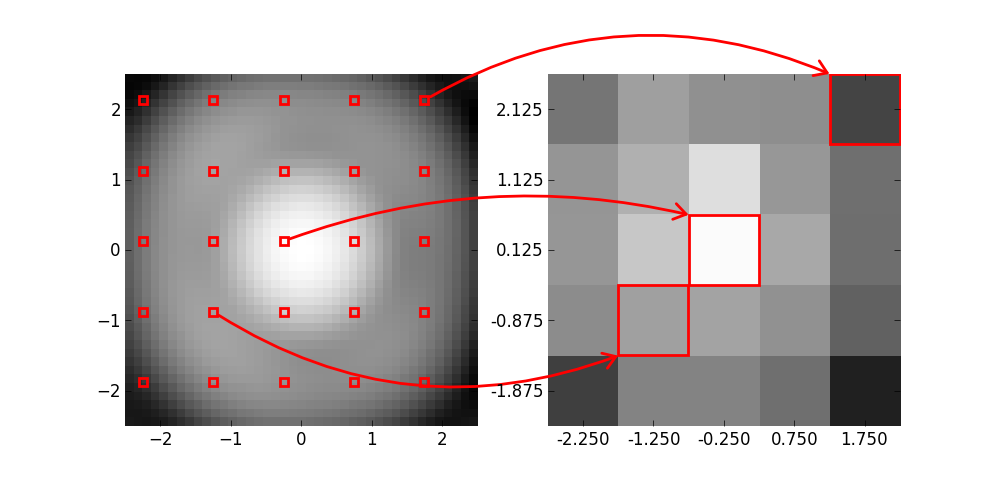
\includegraphics[clip=true, trim=0cm 0cm 0.0cm 0.cm,width=16cm]{../../plots/paper/fig2.png}
\caption{A demonstration of rendering a PSF model for a patch, from the global pixel-convolved PSF 
model.  Shown is the pixel-convolved PSF model on the left, and a PSF model rendered for a $5\time5$
patch on the right.  The sub-pixel shift for the model on the right is (-0.25, 0.125), which given the global 
model's subsampling of 8 means the model on the right can be read exactly off the grid.  Patches with 
sub pixel shifts that do not fall on intervals of 0.125 are generated by cubic spline interpolation.}
\label{fig:psf-generation}
\end{figure}


\subsection{Noise Model}
\label{ssec:noise}

In order to compute the likelihood of our model (described below), we need an estimate of the noise 
present in a given patch.  The MAST pipeline delivers an error estimate for each pixel in the \FLT\ images.   
However, there is a key issue preventing us from using the MAST error estimates.  
For typical astronomical detectors, the variance of 
the data is estimated as a constant (read noise-like term) plus a scaler times the intensity of the pixel 
(gain-like term).  As a consequence, this means a noisy pixel will have an under or over estimated uncertainty depending 
on whether the pixel value is below or above the true value of the flux received.  This has been shown to be 
problematic in the PSF fitting of SDSS data (cite Blanton??).  A better estimate for the uncertainty is 
instead one which scales with the value of the \emph{model}, since we hope the model value is a 
closer estimate of the true pixel intensity.  We therefore adopt a noise model for each patch $\data_i$
as:

\begin{eqnarray}
\var_i =  \sigma_{r}^2 + g \model_i
\quad , 
\label{eqn:model-noflat}
\end{eqnarray}

\noindent where $\sigma_{r}^2$ is `read noise-like' constant scalar and $g$ is a `gain-like' scalar 
which is multiplied by the model.  For simplicity, we set each of these parameters to be the same 
for each data patch.  To set $g$, we took the MAST estimate for the squared error and 
divided by the pixel values.  We then fit a line to pixels with values between 100 and 
400 electrons per second, since such pixels are relatively unaffected by read noise.  We find that 
the slope of this line was consistent with a value of 
$\sim0.01$, but increased sharply for images with exposure time $\lesssim 200$ seconds.  
Nevertheless, we set $g=0.01$ and analyzed the consequences of doing so by examining the 
residuals.  For $\sigma_{r}^2$, we took the median of the MAST squared error estimates.  We find 
significant variation of the median from image to image, but simply set $\sigma_{r}^2=0.05$ since 
it comprises a small contribution to the model of $\var$ for the vast majority of the pixels in our 
patches.

\subsection{Patch Fitting, Optimization, and Outlier Control}
\label{ssec:optimization}

We seek to find the optimal 2D grid pixel-convolved PSF model values which best represent the 
data.  In order to do this we not only need to optimize $N_{psf} \times N_{psf}$ parameters for the 
global PSF model, but we need to find the appropriate amplitudes, backgrounds, and centroids 
for each patch in consideration.  In principle, all these parameters could be put into a standard 
optimization routine in order to find a solution.  In practice, however, we find such a straightforward 
approach to be too costly computationally: optimization is extremely slow given the large number 
of parameters involved, the numerous local minima present, and the lack of analytic derivatives of 
our loss function (due to the non-trivial dependence on our use of 
\texttt{scipy.interpolate.RectBivariateSpline}).  Instead, we use an iterative approach that is an 
Expectation-Maximization optimization of the parameters.  Simply put, for each iteration we first 
hold the current PSF model fixed in order to find the current best centroids for the patches after 
which we hold the centroids fixed and search for the current best update to the PSF.  

At each stage of this optimization procedure (whether searching for centroids or PSF parameters),
we query a likelihood function for the patch which reads in values for the centroid and PSF,
determines the amplitude $A_i$ and background $\bkg_i$ via linear least squares fitting, and 
returns the likelihood for the patch:

\begin{eqnarray}
L_i =  -\frac{1}{2}\left(\ln(\var_i) +  \frac{(\data_i - \model_i)^2}{\var_i} + \ln(2\pi)\right)
\quad .
\label{eqn:patch-likelihood}
\end{eqnarray}

\noindent where we have defined $\model_i$ and $\var_i$ in Sections \ref{ssec:model} and 
\ref{ssec:noise} above.  

Centroid search proceeds by its own sub-optimization, under some model assumptions.  
In particular, we restrict the part of the patch used for the search to the central $5\time5$ region 
of the patch.  This is done to restrict the impact of other sources present in the patch, and 
to speed up computation.  We assume during this that any residual flux present in the central 
region originating from nearby sources is small relative to the flux levels (in this highest S/N) 
region, and can be reasonably accounted for by the background model.  The optimal 
centroids are found by maximizing Equation \ref{eqn:patch-likelihood} using a standard
optimization algorithm, holding the current PSF model fixed.  We find that, lacking analytic 
derivatives, a modified Powell optimization algorithm 
(implemented in \texttt{scipy.optimize.fmin\_Powell}) is particularly efficient for this search.  
When performing any fits to individual patches, we exclude pixels flagged as questionable 
by the MAST/HST team.

Updating the PSF after obtaining new centroids requires some careful consideration.  First, 
we need to address the presence of multiple sources in the majority of the image patches.  As 
stated in Section \ref{ssec:model}, we have restricted our computation to a vary simple model: 
there is just one scaled PSF and a constant background with which we work.  Given that this 
model cannot account for additional sources, the likelihood of many patches will be dominated 
by such errors (and hence may wreck PSF inference outside the central regions of the model), 
we must add some complexity to our patch fitting.  For efficiency, we choose to simply clip ill 
fitting portions of patches using a $\chi^2$ criterion:

\begin{eqnarray}
\chi^2_{i, {\rm clip}} &=& \frac{(\data_i - \model_i)^2}{\var_{i, {\rm clip}}} \quad , {\rm where} \\
\var_{i, {\rm clip}} &=&  \sigma_{r}^2 + g \model_i + q (A_i \psf_i)^2
\quad .
\label{eqn:chi2-clip}
\end{eqnarray}

\noindent  The above $\chi^2$ is the standard $\chi^2$  under the noise model, but with the
variance increase by a factor $q$ times the scaled PSF.  This has the effect of asking how 
discrepant the current model is from the scaled PSF, thus selecting clipping regions where 
the residuals are q times as far from the PSF.  We set $q=1$ for the work here.  We find this 
version of clipping to be fairly robust and quick 
to compute, and we set our clipping criterion to $\chi^2_{i, {\rm clip}} > 3$ during optimization.  As 
an extra precaution, we take masks defined by this criterion and grow them in each direction 
by one pixel.  Because the amount of pixels might be large in crowded fields, we require that 
at least 50\% of the pixels in a patch must not be masked in order to be used in the inference.  
Figures \rf{ADD FIGURES} demonstrate our clipping procedure and the corresponding effect 
on the calculated likelihoods.

With clipping in place, PSF updates proceed as follows.  Upon each iteration, a new list of 
patches is introduced.  After their centroids are found, we calculate numerical derivatives of 
a cost function relative the $N_{psf} \times N_{psf}$ PSF parameters.  This cost function is

\begin{eqnarray}
C = \sum_i -L_i + \lambda \sum_{j, k} \delta_{j, k}
\quad ,
\label{eqn:patch-likelihood}
\end{eqnarray}

\noindent where the first term is a sum over the $L_i$ likelihoods presented in Equation 
\ref{eqn:patch-likelihood}.  The second term is a regularization term we impose on the PSF.
The purpose of this regularization term is to enforce our belief that the PSF ought to be a 
smoothly varying function.  There are many forms this regularization might take, but for this 
work we choose work with the sum of absolute differences between a given PSF model pixel and its 
nearest neighbors.  As such, we define $\delta_{j, k}$ to be this sum of differences for the pixel 
in the j-th row and k-th column and $\lambda$ is a constant that sets the strength of the regularization.

Taking the derivatives of this cost function using the data presented at a given iteration 
gives us directions up or down we might move pixels in the PSF model to move towards the 
optimum.  From here, one might simply search for the multiplicative constant that we can 
rescale the derivatives by and subtract off from the current model, which optimizes the likelihood 
of the data used in the iteration.  This, however, leads to over fitting - by tuning the PSF 
update to that particular chunk of data, the new PSF will tend to not generalize well to new 
patches.  Instead, we search for the constant that optimizes the likelihood of a separate, 
validation list of random patches.  This validation list is never used during optimization to compute
derivatives for PSF updates, and hence the likelihood of these patches reflect how well the 
new PSF will generalize.  To ensure robustness, we insist that the number of validation patches 
is large (typically a few thousand), and that many optimizations are run with different validation 
sets.  The final PSF is the mean of the different validation runs.

While we believe our selection of patches from the \FLT\, images is actually quite good, we fold in 
two important additional prescriptions for removing patches that may still contain non-stellar sources 
or other problematic issues.  First, when we compute the centroids we examine the likelihood of the 
patches and discard a small fraction of patches with the worst likelihoods.  Second, when updating 
the PSF we want the validation likelihood to be robust.  For this, we consider as our score the 
mean of the patch likelihoods in inner 68\% of the validation likelihood distribution.

\section{Results}

\section{Discussion}

We perform very well.

We are the only publicly available PSF and software!
(Maybe here or in an appendix give some example command-line operation.)

It would be good to have more data;
  what could we do if we did?

The problem is sparse in structure;
  we could have made much more use of that sparsity to speed things up.

We had various knobs to turn; we set them heuristically.
What would be better?

We ignored various issues: source spectrum, inter-pixel sensitivity, ...

We worked in a very knowledge-free way;
  we could have used our prior knowledge better.
For instance, we could have started by subtracting out the pixel-convolved fourier transform of the entrance aperture;
  then we would only have been fitting residuals.
Even better would be to start with a prior PDF over PSFs;
  that's a dream.

We only fit the pixel-convolved PSF.
Once again, why is this a good idea?
Once again, how should this be used by other users?
How could one infer the optical PSF from these results?

\clearpage

\bibliographystyle{apj}
\begin{thebibliography}{44}

\bibitem[{{Anderson \& King} (2006){Anderson} \& {King}}]{anderson06}
{Anderson}, J., \& {King}, I. 2006, Instrument Science Report ACS 2006-1

\bibitem[{{Bertin \& Arnouts} (1996){Bertin} \& {Arnouts}}]{bertin96}
{Bertin}, E. \& {Arnouts}, S. 1996, A\&AS, 117, 393

\end{thebibliography}

\end{document}
